\section{Projekt graficznego interfejsu użytkownika}
    Interfejs graficzny będzie przedstawiać w czterech wybieralnych zakładkach dwa silosy, na który prezentowane będą następujące elementy:
        \begin{itemize}
            \item widok wszystkich parametrów,
            \item widok wypełnienia,
            \item widok temperatury,
            \item widok wilgotności,
        \end{itemize}
    Ponadto dostępna będzie również piąta zakładka, prezentująca na wykresach dane historyczne.
    
    W kolejnych podpunktach zostaną przedstawione schematyczne grafiki prezentujące poszczególne widoki aplikacji
    na dane parametry.

    \subsection{Widok wszystkich parametrów}
        \begin{figure}[H]
            \centering
            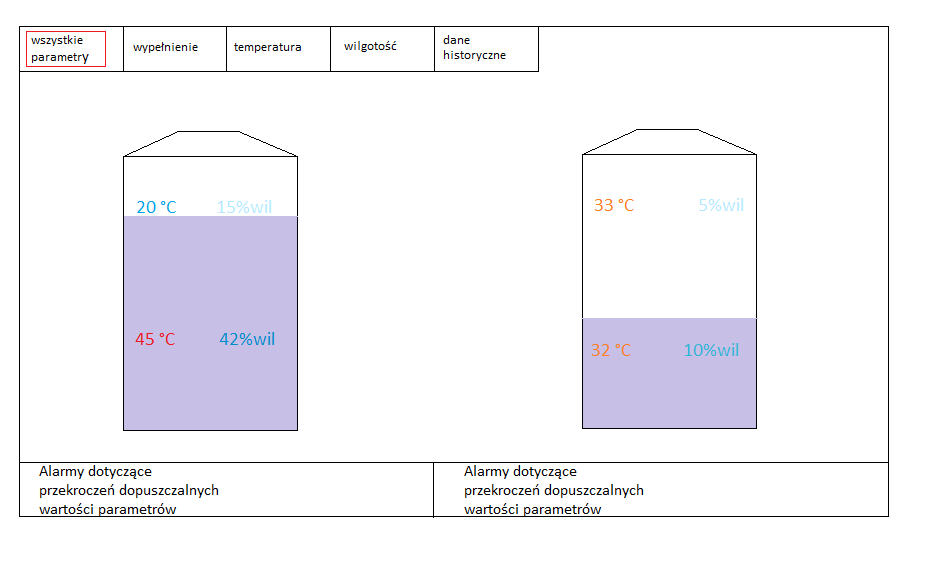
\includegraphics[width = \textwidth]{obrazy/projekt_grafiki/all.png}
            \caption{Widok na wszystkie parametry}
            \label{fig: all}
        \end{figure}
        Rysunek \ref{fig: all} prezentuje idee poglądu na wszystkie parametry dotyczące silosów. Aby wybrać ten widok,
        w górnym pasku należy zaznaczyć opcje ,,wszystkie parametry''. Wypełnienie silosu symbolizowane jest kolorem. 
        w sposób tekstowy zaprezentowane zostaną wartości odczytane z czujników temperatury i wilgotności. Kolor czcionki
        będzie symbolizował wartość parametru, np. czerwony kolor czcionki będzie występował wraz ze wskazaniem temperatury 
        przekraczającej poziom alarmowy. Pod silosami znajdują sie pola przeznaczone do informowania o zaistniałych alarmach.
    \subsection{Widok wypełnienia}
        \begin{figure}[H]
            \centering
            \includegraphics[width = \textwidth]{obrazy/projekt_grafiki/wypełnienie.png}
            \caption{Widok na wypełnienie silosów}
            \label{fig: wypelnienie}
        \end{figure}

        Rysunek \ref{fig: wypelnienie} prezentuje idee poglądu na wypełnienie silosów. Aby wybrać ten widok,
        w górnym pasku należy zaznaczyć opcje ,,wypełnienie''. Wypełnienie silosów symbolizowane będzie zapełnieniem
        obrysu silosów kolorem. Niski poziom będzie sygnalizowany na czerwono, poziomy bliskie połowy odcieniami żółtego,
        zbliżając się do maksymalnego poziomu kolor będzie stawał się zielony. Dodatkowo widoczna będzie informacja 
        o zapełnieniu silosów wyrażona w procentach.
    \subsection{Widok temperatury}
        \begin{figure}[H]
            \centering
            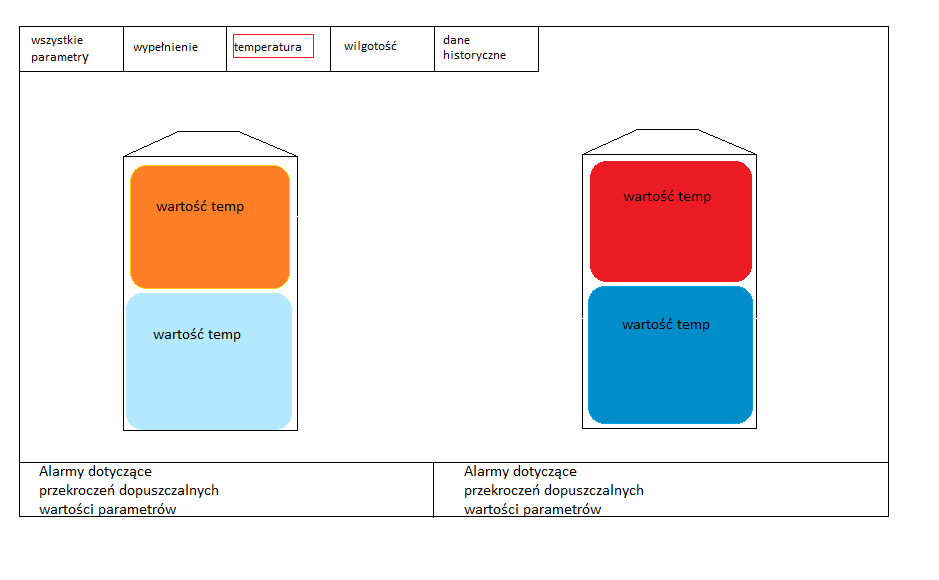
\includegraphics[width = \textwidth]{obrazy/projekt_grafiki/temperatura.png}
            \caption{Widok na temperature wewnątrz silosów}
            \label{fig: temperatura}
        \end{figure}

        Rysunek \ref{fig: temperatura} prezentuje idee poglądu na temperature wewnątrz silosów. Aby wybrać ten widok,
        w górnym pasku należy zaznaczyć opcje ,,temperatura''. Temperatura symbolizowana będzie poprzez gradient kolorów,
        postały na podstawie odczytu temperatury z czujników. Odcienie niebieskiego będą symbolizować niskie temperatury,
        odcienie żółto-pomarańczowe średnie, a czerwone wysokie. Dodatkowo temperatura będzie prezentowana w formie 
        tekstowej.
    \subsection{Wilgotność}
        \begin{figure}[H]
            \centering
            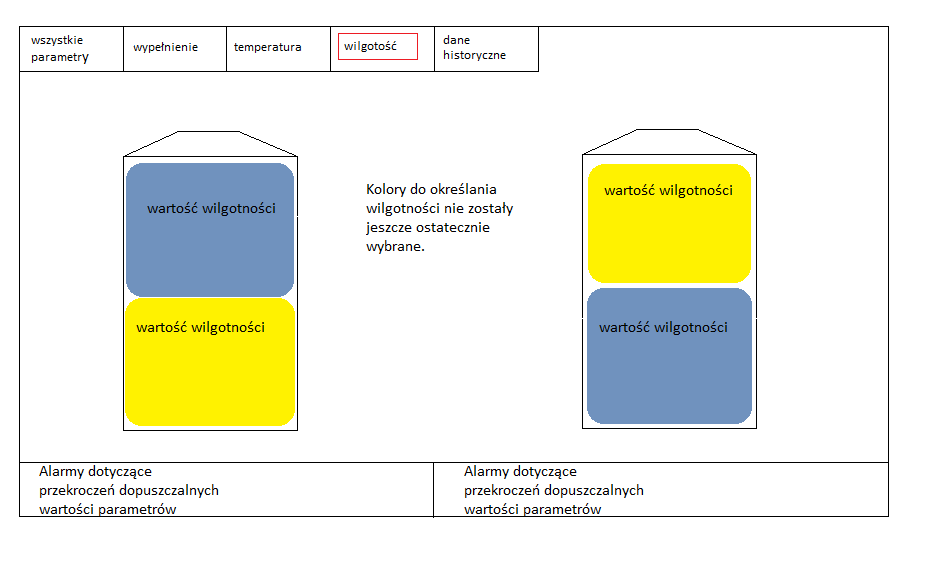
\includegraphics[width = \textwidth]{obrazy/projekt_grafiki/wilgotność.png}
            \caption{Widok na wilgotność wewnątrz silosów}
            \label{fig: wilgotnosc}
        \end{figure}
        Rysunek \ref{fig: wilgotnosc} prezentuje idee poglądu na wilgotność wewnątrz silosów. Aby wybrać ten widok,
        w górnym pasku należy zaznaczyć opcje ,,wilgotność''. Wilgotność symbolizowana będzie poprzez gradient kolorów,
        postały na podstawie odczytu wilgotności z czujników. Nie ustalono jeszcze kolorystyki symbolizującej wilgotność, na grafice \ref{fig: wilgotnosc} kolory zostały wybrane przypadkowo. Dodatkowo wilgotność będzie prezentowana w formie 
        tekstowej.

    \subsection{Dane historyczne}
        \begin{figure}[H]
            \centering
            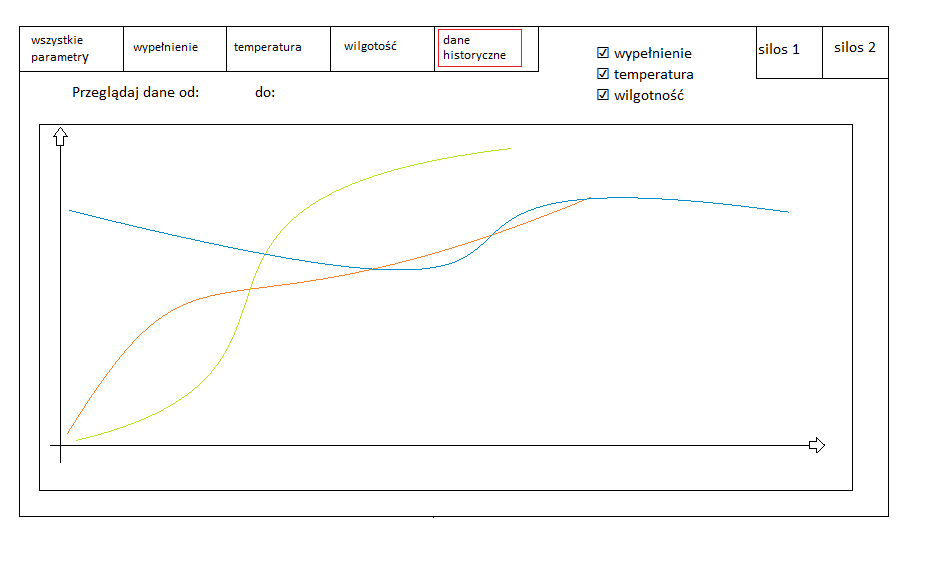
\includegraphics[width = \textwidth]{obrazy/projekt_grafiki/wykresy.png}
            \caption{Widok na dane historyczne}
            \label{fig: dane historyczne}
        \end{figure}
        Rysunek \ref{fig: wilgotnosc} prezentuje idee poglądu na dane historyczne silosów. Aby wybrać ten widok,
        w górnym pasku należy zaznaczyć opcje ,,dane historyczne''. Widok ten przedstawia nam wykresy danych zapisanych i przechowanych przez aplikacje.
        Wykresy można poddać następującym modyfikacją:
        \begin{itemize}
            \item wybór silosu, którego dane chcemy wyświetlić,
            \item wybór danych, które mają zostać wyświetlone,
            \item wybór okresu czasu, z którego mają zostać zaprezentowane  dane.
        \end{itemize}
        